
%% simulation.tex

% Section: EVALUATION
% NOTE: Evaluation section contains all subsections = setup, results, evaluation

\section{Performance Evaluation}
\label{sec__incentivise_evaluation}

In order to assess the suitability of the proposed effort-based mechanism
to community network clouds, 
we need to study how it impacts the efficiency of the system,
and how fair it is to the users with different resource capacities.
As compared to contribution-based mechanisms, which reward the users 
in terms of the total resources they contribute to the system,
effort-based incentives may put high contributors at slight disadvantage,
when they reward the users with low capacities.
So effort-based mechanisms need careful design in order to maintain high system utilisation,
and at the same time ensuring fairness for the users with different level of contributions.

In the following, we evaluate the mechanisms first through simulation experiments (\Cref{sec__incentivise_evaluation_simulation}),
and then through a prototype deployed in a testbed 
with real community network nodes (\Cref{sec__incentivise_evaluation_prototype}).
Our results show that effort-based mechanisms apply well to the context of community network clouds.

\subsection{Evaluation with Simulation Experiments}
\label{sec__incentivise_evaluation_simulation}

We evaluate the impact of the effort-based incentive mechanism through simulation experiments 
that cover resource regulation on a larger scale across multiple SN zones 
covering both local and federated community cloud scenarios.

%%%%%%%%%%%%%%%%%%%%%%%%%%%%%%%%%%%%%%%%
\subsubsection{Experiment Setup}

We simulate a community network comprising of 1000 nodes which is divided into 100 zones and each zone has one SN and nine ONs.
The zones are distributed in a small world topology where each zone is neighbour to 10 other zones.
This approximation holds well for real world community networks as, for example, topology analysis of Guifi.net~\cite{Vega2012} shows that the ratio of super node to ordinary nodes is approximately 1 to 10. 
Each ordinary node in the simulation can host a number of VM instances that allows users' applications to run in isolation.
Nodes in the zone have two main attributes, one is capacity which is the number of available VM instances, and other is sharing behaviour which is how many instances are shared with other nodes.
Table~\ref{tab:ONconf} shows the different configurations for each of the nine ONs in each zone.
Nodes with low, medium and high capacity host 3, 6 and 9 VM instances respectively and they exhibit selfish, normal or altruistic behaviour sharing one-third, two-thirds or all of their VM instances.
For example, node ON2 has medium capacity with 6 instances and exhibits selfish behaviour reserving 4 instances for itself and contributing only 2 to the system.

\begin{table}[tbp]
\renewcommand{\arraystretch}{1.3}
\footnotesize
\centering
     \caption{Configuration for each node in a zone with shared and total instances}
    \begin{tabular}{@{} cc c c c c @{}}
    \hline
    {Node Behaviour} & {Shared} & Small capacity & Medium capacity & Large capacity   \\  \hline
    {Selfish} & 33\% 	& ON1 (1/3) & ON2 (2/6) & ON3 (3/9) & \\ 
	{Normal} & 66\% 	& ON4 (2/3) & ON5 (4/6) & ON6 (6/9) & \\ 
	{Altruistic} & 100\%& ON7 (3/3) & ON8 (6/6) & ON9 (9/9) & \\ \hline
    \label{tab:ONconf}
    \end{tabular}
\end{table}

When the experiment runs, the nodes are given initial credit in proportion to their capacity.
Nodes make requests for resources proportional to their capacity asking for two-thirds of their capacity.
For instance nodes with capacity of 3, 6 and 9 VM instances request 2, 4 and 6 instances respectively.
Nodes request instances for fixed duration and after transaction is complete wait briefly before making further requests.
We have implemented the simulator in Python.

%%%%%%%%%%%%%%%%%%%%%%%%%%%%%%%%%%%%%%%
\subsubsection{Ratio of Successful Requests}

Table~\ref{tab__success_ration_effort_contrib} shows the success ratio for requests 
made by different nodes analysed both with the effort-based and contribution-based incentive mechanisms. 
We first notice that the success ratio values decrease as the capacity of the nodes increases. 
This is explained by the fact that nodes with greater capacity request more instances, 
and so have a higher chance of getting rejected 
either because there are not many resources available in the system 
or because the requesting nodes do not have sufficient credit.
However, when comparing the success ratio for nodes as their capacity increases, we observe that there is not a great variation.
For instance, for the normal sharing behaviour the values range from 66\% to 97\% for contribution-based incentives, but from 86\% to 90\% for effort-based incentives.
This is explained by the fact that contribution-based approach does not take heterogeneity of nodes into account, 
and penalises nodes with low capacity as they cannot contribute as much to the system as others.
These results indicate that effort-based incentives ensure \emph{fairness} in the system, 
since the nodes with the same sharing behaviour are treated equally irrespective of their capacity.

\begin{table}[tbp]
\renewcommand{\arraystretch}{1.3}
\footnotesize
\centering
  \caption[Success ratio for nodes with different configurations]{Success ratio for nodes with different configurations (effort vs contribution)}
    \begin{tabular}{@{} cc c c c c @{}}
    \cline{1-5}
     {Node Behaviour} & {Incentives} & Small capacity & Medium capacity & Large capacity   \\ \hline 
     {\multirow{2}{*}{Selfish}} &
	 {effort-based} & 54\% & 53\% & 50\% & \\ 
	 {} &
	 {contribution-based} & 66\% & 59\% & 39\% & \\ \hline
 	 {\multirow{2}{*}{Normal}} &
	 {effort-based} & 90\% & 91\% & 86\% & \\ 
	 {} &
	 {contribution-based} & 97\% & 77\% & 66\% & \\ \hline
 	 {\multirow{2}{*}{Altruistic}} &
	 {effort-based} & 97\% & 94\% & 86\% & \\ 
	 {} &
	 {contribution-based} & 97\% & 85\% & 65\% & \\ \hline
    \label{tab__success_ration_effort_contrib}
    \end{tabular}
\end{table}

%%%%%%%%%%%%%%%%%%%%%%%%%%%%%%%%%%%%%%%
\subsubsection{Breakdown of Request Responses}

Figure~\ref{fig:req_breakdown} shows the overall breakdown of successful and rejected requests across all the zones,
where there are many more successful requests than rejected ones. 
The success ratio is slightly better for effort-based incentives.
Moreover, contribution-based mechanism has greater share of requests rejected because of lack of credit,
while very few requests are rejected because of a lack of resources.
This indicates that the effort-based incentive mechanism improves efficiency as more resources are utilised. 
In addition to this observation, the majority of the requests are fulfilled using resources from the local zone with very few requests forwarded to other zones. 

\begin{figure}[tbp]
   \centering
   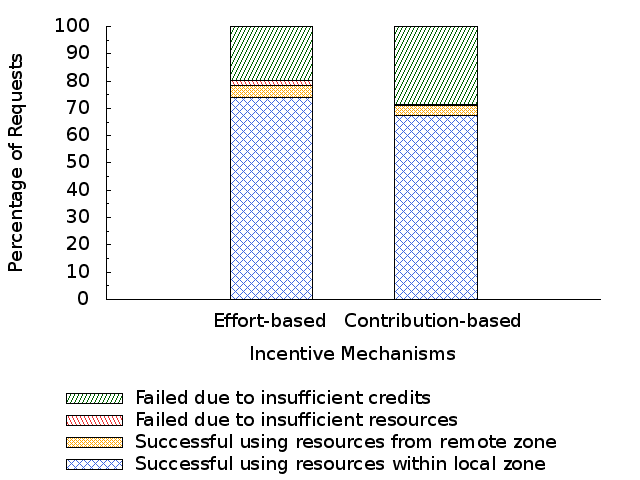
\includegraphics[width=0.65\textwidth,keepaspectratio]{graph_requestRatio}
   \caption[Breakdown of outcome of requests]{Breakdown of outcome of requests with effort and contribution based mechanisms}
   \label{fig:req_breakdown}
\end{figure}

%%%%%%%%%%%%%%%%%%%%%%%%%%%%%%%%%%%%%%%
\subsubsection{Resource Utilisation}

Figure~\ref{fig:res_util} shows the proportion of resources utilised in the system 
along the execution of a 24 minutes experiment for effort and contribution based approaches. 
In the beginning, all nodes have enough credit and the resource utilisation is high. 
Then it drops to below 60\% at around the 12th minute, 
and keeps fluctuating for a while. 
Afterwards, since most of the nodes have completed their transactions and consumed their credits, 
the utilisation decreases significantly. 
The effort-based approach though achieves a higher resource utilisation during that time. 

The results also point to a possible load imbalance issue since as the experiment progresses 
the large capacity nodes may accumulate the credit, lowering the percentage of used resources over time. 
Many nodes are left with insufficient credit to consume resources. 
One approach to overcome this issue is to supply all the nodes 
with a limited fixed amount of credit at regular intervals, which will keep the resource utilisation high.

%% Graph 
\begin{figure}[tbp]
   \centering
   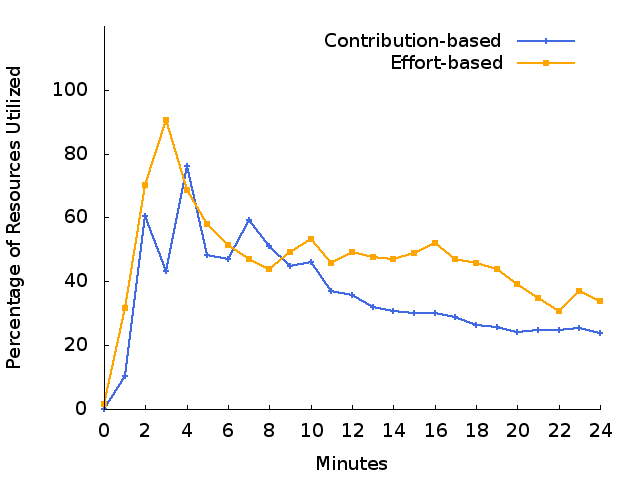
\includegraphics[width=0.65\textwidth,keepaspectratio]{graph_resourceUtil}
   \caption{Resource utilisation}
   \label{fig:res_util}
\end{figure}
